\section{Logical design - Relational model}

\begin{theorem}
    {Physical and logical data independence}
    \begin{itemize}
        \item \textbf{Physical}: changes to the physical storage of the database do not affect the logical schema or the views of the data.
        \item \textbf{Logical}: changes to the logical schema do not affect the physical storage of the database or the views of the data.
    \end{itemize}
\end{theorem}

\begin{definition}
    {Relation (Schema)}
    A \textbf{relation} (or table) is a set of \textbf{tuples} (or rows) having the same \textbf{attributes} (or columns).

    Relations (schemas) are represented as: $R(A_1A_2 \ldots A_n)$.
\end{definition}

\begin{knBox}
    {Relation instance}
    A set of tuples (rows) that satisfy the relation schema.

    \textbf{Degree/arity}: Number of attributes;
    \textbf{Cardinality}: Number of tuples;
\end{knBox}

\subsection{Relational models in SQL}

Basic table operations:

\begin{itemize}
    \item \verb|CREATE TABLE <table_name> (...);|
    \item \verb|DROP TABLE <table_name>;|
    \item \verb|ALTER TABLE <table_name> ADD <column_name> <data_type> [constraints];|
\end{itemize}

Example:

\begin{verbatim}
    CREATE TABLE Grade (
        sid INTEGER,
        dept CHAR(4), 
        mark INTEGER NOT NULL,
        some_other_unique_attribute CHAR(4),   
        PRIMARY KEY (sid,dep),
        FOREIGN KEY (sid) 
            REFERENCES Student
            ON DELETE CASCADE
            ON UPDATE CASCADE,
        FOREIGN KEY (dept) REFERENCES Course(dept)
            ON DELETE SET NULL
            ON UPDATE CASCADE
        UNIQUE (some_other_unique_attribute)
    );
\end{verbatim}

\begin{definition}
    {Integrity constraints}
    Conditions are must be true for any instance of the database

    \begin{itemize}
        \item \texttt{... NOT NULL}: the column cannot be NULL
        \item \texttt{UNIQUE(attr)}: the column cannot have duplicate values
        \item \texttt{PRIMARY KEY (attr,)}: the column is the primary key of the table
        \item \texttt{FOREIGN KEY (attr,) REFERENCES Table(attr,)}: the column is a foreign key of the table
    \end{itemize}

\end{definition}

\begin{definition}
    {Referential integrities}

    Referential integrity constraints are used to enforce the relationship between tables.

    \begin{itemize}
        \item \texttt{ON DELETE ...}: what to do when the referenced tuple is deleted
        \item \texttt{ON UPDATE ...}: what to do when the referenced tuple is updated
    \end{itemize}

    The following options are available:

    \begin{itemize}
        \item \texttt{CASCADE}: delete or update the tuples in the referencing table when the referenced tuple is deleted or updated.
        \item \texttt{SET NULL}: set the foreign key values in the referencing table to NULL when the referenced tuple is deleted or updated.
        \item \texttt{SET DEFAULT}: set the foreign key values in the referencing table to their default values when the referenced tuple is deleted or updated.
        \item \texttt{NO ACTION}: reject the delete or update operation on the referenced tuple if there are any matching tuples in the referencing table.
    \end{itemize}
\end{definition}

\subsection{ER Constraints to relational model}

Refer to \ref{sec:constraints}.

\begin{theorem}
    {Key constraints}
    \begin{itemize}
        \item \textbf{1-1 / 1-M}
              \begin{itemize}
                  \item $\forall$"1"key $\to$ Foreign key on other table, OR;
                  \item +relation, $\forall$"1"key $\to$ Foreign key UNIQUE, pKey = all attrs
              \end{itemize}
        \item \textbf{M-M}: +relation, $\forall$"M"key $\to$ Foreign key, pKey = all attrs
    \end{itemize}

    \tcblower

    Consider ER diagrams, underlined are pKeys, bold are foreign keys:
    \begin{itemize}
        \item \texttt{[A](\underline{a})} $\rightarrow$ <R> $\leftarrow$ \texttt{[B](\underline{b})}:
              \begin{itemize}
                  \item \texttt{RA(\underline{a}, \textbf{b}); RB(\underline{b}, \textbf{a})}
                  \item \texttt{RA(\underline{a}); RB(\underline{b}); RAB(\textbf{\underline{a}} UNIQUE, \textbf{\underline{b}} UNIQUE)}
              \end{itemize}
        \item \texttt{[A](\underline{a})} -- <R> -- \texttt{[B](\underline{b})}:
              \begin{itemize}
                  \item \texttt{RA(\underline{a}); RB(\underline{b}); RAB(\textbf{\underline{a}}, \textbf{\underline{b}})}
              \end{itemize}
    \end{itemize}
\end{theorem}

\begin{theorem}
    {Total participation constraint}
    Consider key constraints:
    \begin{itemize}
        \item \textbf{1-1 / 1-M (Total participation on M side)}: Foreign key NOT NULL
        \item \textbf{M-1 (Total participation on 1 side) / M-M}:  We cannot enforce total participation on data level directly. (Required triggers / application-level logic)
    \end{itemize}
\end{theorem}

\begin{theorem}
    {Weak entities / Belongs to}
    +relation for weak entity relation, ownerKey $\to$ Foreign key, pKey = \{ownerKey, partialKey\}

    \tcblower

    Consider ER: \texttt{\textbf{[A]}(partialKey)} $\rightarrow$ \textbf{<R>} -- \texttt{[B](\underline{ownerKey})}:

    \texttt{RA(\underline{partialKey}, \underline{\textbf{ownerKey}}); RB(\underline{ownerKey})}

    Consider ER: \texttt{\textbf{[A]}(partialKey)} $\rightarrow$ \textbf{<R>} $\leftarrow$ \texttt{[B](\underline{ownerKey})}:

    \texttt{RA(partialKey NOT NULL, \underline{\textbf{ownerKey}}); RB(\underline{ownerKey})}
\end{theorem}

\begin{theorem}
    {Generalization / Specialization / IsA}

    \begin{itemize}
        \item +relationA for super class, pKey = pKey of super class
        \item +relationN for subclass (with the additional attrs), pKeyA $\to$ Foreign key, pKey = \{ pKeyA \}
    \end{itemize}

    \tcblower

    Consider ER: \texttt{[General](\underline{a})} -- $\triangle$IsA -- \texttt{[Specific](b,c,d)}:

    \texttt{RA(\underline{a}); RB(\underline{\textbf{a}}, b, c, d)}
\end{theorem}

\begin{theorem}
    {Aggregation}

    +relation for aggregated relationship set, setup keys as normal.
\end{theorem}

\subsection{Relational model to ERD}

\begin{itemize}
    \item Foreign keys should not be converted to attributes!
\end{itemize}

% \tcblower

% \begin{center}
%     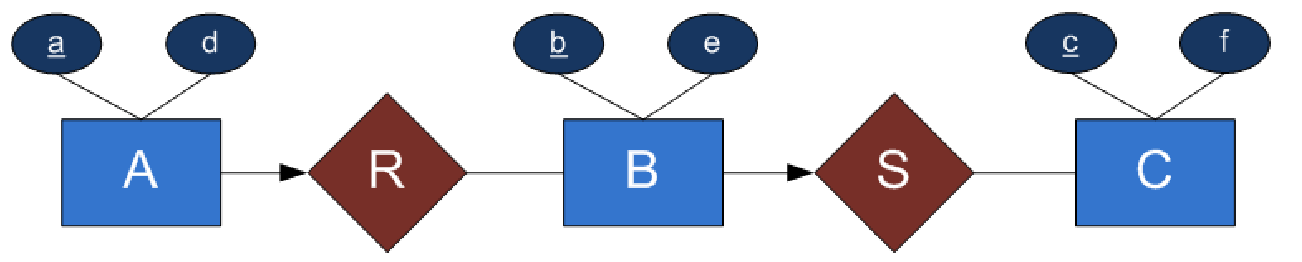
\includegraphics[width=0.7\textwidth]{images/3-1.png}
% \end{center}

% The relational schema for the above ER diagram is:

% \begin{center}
%     AR(\underline{a}, \underline{\textbf{b}}, d), BS(\underline{b}, \underline{\textbf{c}}, e), C(\underline{c}, f)
% \end{center}

% Where \textit{underlined} are primary keys of the respective tables, and \textit{bold} are foreign keys.